<<<<<<< HEAD
\chapter{Módulo firmware}

En este capítulo se expone el trabajo relacionado con la programación a bajo nivel realizada sobre la electrónica propuesta en el capítulo anterior.

Dado que la electrónica se basa en la plataforma Arduino, tal programación se realiza usando su propio lenguaje basado en C/C++.

El firmware es el encargado de detectar y controlar cambios en los estados de los periféricos y sensores que se produzcan por cualquier evento, interno o externo.


\section{Diseño y Análisis}
\subsection{Requisitos funcionales}

Pasamos a determinar los requisitos que debe satisfacer nuestro firmware.


Los requisito funcionales están estrechamente relacionados con los requisitos propuestos en el anterior capítulo. 

\begin{itemize}
	
	\item \textbf{RF-1.}: Controlar motor paso a paso:
	\begin{itemize}
		\item \textbf{RF-1.1.}: Controlar la dirección.
		\item \textbf{RF-1.2.}: Controlar velocidad.
		\item \textbf{RF-1.3.}: Controlar microstepping, para conseguir la máxima resolución en los pasos. \cite{micros}
		
	\end{itemize} 	
	\item \textbf{RF-2.}: Mostrar información del sistema mediante una pantalla LCD.
	
	\item \textbf{RF-3.}: Modificar parámetros de forma manual
	\begin{itemize}
		\item \textbf{RF-3.1.}: Modificar velocidad.
		\item \textbf{RF-3.2.}: Modificar mover \texttt{n} pasos por pulsación.
	\end{itemize}	
	\item \textbf{RF-4.}:Ejecutar funciones de movimiento del motor desde una botonera o control manual.
	\begin{itemize}
		\item \textbf{RF-4.1.}: Ejecutar función de movimiento continuo en la dirección deseada.
		\item \textbf{RF-4.2.}: Ejecutar función de movimiento (\texttt{n} pasos) en la dirección deseada. 
	\end{itemize}
	
	\item \textbf{RF-5.}: Monitorizar temperatura y mostrar aviso cuando se detecte un cambio.
	
	\item \textbf{RF-6.}: Controlar límites físicos en el desplazamiento de las partes mecánicas del enfocador.  
	
	\item \textbf{RF-7.}: Hacer las sesiones persistentes, recordando los estados después de una desconexión. 
	
	\item \textbf{RF-8.}: Modificar y consultar los estados del dispositivo, mediante una API.
	
	\item \textbf{RF-9.}: Se debe permitir el encender y apagar la retro-iluminación de la pantalla.
\end{itemize}

\subsection{Requisitos no funcionales}

\begin{itemize}
		\item \textbf{RNF1.}: El sistema debe responder a las ordenes en tiempo real y de forma interactiva.
		
		\item \textbf{RNF2.}: La velocidad de giro del motor no debe estar condicionada por la velocidad del microcontrolador.
		
		\item \textbf{RNF3.}: La pantalla LCD debe refrescarse solo cuando existan cambios en los datos a presentar. 
		
		\item \textbf{RNF4.}: La comunicación serie debe ser robusta y tolerante y el protocolo debe ser tolerante a perdida de mensajes.
		
		\item \textbf{RNF5.}: El protocolo serie debe ser flexible y permitir extenderse con nuevos mensajes o cambiar por completo el repertorio de los mismos.
		
		\item \textbf{RNF6.}: La escritura en memoria EEPROM tiene que hacerse de forma eficiente y limitando el número de escrituras en los posible, dado que es un elemento que se deteriora.
		
\end{itemize}

Todo ello debe implementarse con una buena calidad de código permitiendo añadir más módulos y consiguiendo que la API sea ampliable a nuevos comandos.

Con la experiencia y el trabajo realizado nos hemos ido familiarizándonos con la plataforma, conociendo nuevas bibliotecas de utilidad, nuevos periféricos, así como mediante sesiones de \textbf{refactorización} se consigue hacer el código más \textbf{limpio}, \textbf{mantenible} y \textbf{modular}. 

Las entrada al sistema hardware de enfoque, proviene de cuatro fuentes.

\begin{enumerate}
	\item Los sensores inherentes al dispositivo.
	\item Variables de configuración o estados de la sesión anterior. 
	\item Controles manuales, ya sean botoneras o potenciómetros.
	\item Controles remotos que llegan al dispositivo en forma de comandos por el puerto serie.
\end{enumerate}

Por tanto el sistema, se descompone en los siguiente módulos.

\begin{itemize}
	\item \textbf{Módulo para el control de motores}, encargado de actuar sobre el motor, de forma precisa. Debe controlar variables y estados tales como  posición actual, velocidad, aceleración, sentido de giro y respetando los módulos de sensores y control. 
	
	\item \textbf{Módulo de sensores}, que se ocupa de manejar la información proveniente de sensores externos, tales como sensores finales de recorrido o un sensor de temperatura. Debe controlar el estado de dichos sensores (presencia de un tope que limite el movimiento en uno de los sentidos, temperatura de último enfoque y actual).
	
	\item \textbf{Módulo control manual}, que se encarga de leer los diferentes botones y potenciómetros, con los que el usuario puede manejar directamente el dispositivos. Tenedremos estados para cada uno de los botones y los comunicara al módulo de motores. Si cambia la configuración o sensor lo comunicará por puerto serie y/o módulo de visualización LCD.
	
	\item \textbf{Módulo de visualización}, que se encargará de pintar la información en la pantalla LCD.
	
	\item \textbf{Módulo de control remoto}, su trabajo será estar a la escucha de los posibles comandos que puedan llegar por el puerto serie y comunicarlo al modulo que corresponda. 
	
	\item \textbf{Modulo de configuración y almacenamiento de sesión}, que se encargará de manejar todas las variables de configuración, así como almacenarlos en EEPROM para que se mantengan de forma persistente para la próxima sesión de trabajo.
	
\end{itemize}



\section{Arquitectura firmware}


Para la programación del firmware se sigue un diseño donde se diferencian cuatro grandes bloques funcionales. 


\begin{itemize}
	\item \textbf{Initializer}: Método \texttt{init()} de la API de Arduino, que se ejecuta en primera instancia, prepara todo el entorno de ejecución, declarando las entradas y salidas, reservando memoria, iniciando interrupciones, así como ejecutar rutinas como cargar sesión anterior o crear instancias a modo de \textit{singleton} para los manejadores de los diferentes periféricos. 
	
	\item \textbf{Controlador principal}: Bucle principal que se ejecuta periódicamente (el periodo no se puede modificar y lo marca la velocidad del reloj del micro), por lo tanto no es adecuado ejecutar rutinas con restricciones temporales fuertes. Se corresponde con el método \texttt{loop()} de la API de Arduino y se ocupa de manejar la mayoria de las entradas y salidas.
	
	\item \textbf{Interrupciones software}, se ejecutan en un periodo marcado por un \textit{timer}, similar al loop pero con periodos fijos. Se usa para rutinas con restricciones temporales fuertes.
	
	\item \textbf{Interrupciones hardware}, se ejecutan rutinas ligadas directamente a eventos de entrada y salida en alguno de los pines habilitados para tal fin. 
\end{itemize}

Podemos ver un diagrama simplificado en la figura~ \ref{fig:arquitectura_firmware}.

\begin{figure}[h]
\centering
\includegraphics[width=0.9\linewidth]{../images/firmware}
\caption[Gráfico de flujos de ejecución]{Flujos de ejecución del firmware y los eventos que activan los flujos.}
\label{fig:arquitectura_firmware}
\end{figure}


\section{Módulo de control de motores}

Para conseguir precisión en el control del motor, hacemos uso de la biblioteca \textbf{AccelStepper} \cite{accelstp}, compatible con el controlador usado POLOLU A4988. Sus características son las siguientes:

\begin{itemize}
	\item Soporta aceleración y desaceleración.
	\item Soporta múltiples motores paso a paso, de forma concurrente.
	\item La API no añade bloqueos o retardos por delays().
	\item Soporta diversos tipos de controladores.
	\item Permite velocidades muy lentas.
	\item La API es extensible.
\end{itemize} 

En el fragmento de código \ref{lst:accelstepper_sample} podemos ver un ejemplo de uso sencillo de esta biblioteca.

\begin{lstlisting}[language=cpp, caption={Ejemplo de uso de AccelStepper, biblioteca usada para controlar motores paso a paso},label={lst:accelstepper_sample}]
#include <AccelStepper.h>
// Declaramos pines digitales donde se conecta el controlador.
#define PINDIR 3
#define PINSTEP 2

AccelStepper motor(1, PINSTEP, PINDIR);

void setup() {
	// Asigna velocidad.
	motor.setMaxSpeed(200);
	// Asigna Aceleración.
	motor.setAccelerration(1000);
}
void loop() {
	// Inicia movimiento.
	motor.run();
	// Asigna posición de destino.
	motor.moveTo(3000);
}

\end{lstlisting}


\section{Módulo de control remoto}

Para comunicar el dispositivo con las aplicaciones que se ejecutan en un ordenador o servidor, hacemos uso de una comunicación mediante puerto \textbf{serie}. Para ello creamos un protocolo basado en comandos y parámetros. 

El puerto serie envía la información mediante una secuencia de bits por los conectores, RX (recepción) y TX (transmisión). En Arduino UNO y Mini Pro los pines empleados son 0 (RX) y 1 (TX). En nuestro caso la comunicación utilizará una velocidad de transferencia de 9600 baudios.

La nomenclatura seguida todos los comandos tiene el siguiente formato: 


\begin{center}
	\texttt{COMANDO?ARGUMENTO1?ARGUMENTO2 } 
\end{center}

Y la lista de comandos completa que hemos definido se puede encontrar en la tabla~\ref{tab:comandos}.

\begin{table}[]
	\centering

	\begin{tabular}{|l|l|l|}
		\hline
		Comando   & Parámetro             & Descripción                                                                                                 \\ \hline\hline
		AINIT     & -                     & Iniciar modo funcionamiento Ardufocuser.                                                                    \\ \hline
		AMODE     & MODE (int)            & Establecer modo de funcionamiento.                                                                          \\ \hline
		AG        & POSITION (int)        & \begin{tabular}[c]{@{}l@{}}Mover enfocador hasta posición\\  pasada como dato.\end{tabular}                 \\ \hline
		APOSITION & -                     & Solicitar posición actual del enfocador.                                                                    \\ \hline
		ATEMP     & -                     & Solicitar temperatura de la lente.                                                                          \\ \hline
		AMICRO    & MICRO (int)           & Establecer multiplicación del micropaso.                                                                    \\ \hline
		AFINE     & STEEP PER PULSE (int) & \begin{tabular}[c]{@{}l@{}}Establecer pasos que da el enfocador\\  por cada pulso.\end{tabular}             \\ \hline
		ASPEED    & SPEED (int)           & Establecer la velocidad del movimiento.                                                                     \\ \hline
		AACC      & ACCELERATION (int)    & Establecer la aceleración del movimiento.                                                                   \\ \hline
		AR        & POSITION (int)        & \begin{tabular}[c]{@{}l@{}}Fijar posición relativa del enfocador\\  en un valor personalizado.\end{tabular} \\ \hline
		AHLIMIT   & -                     & \begin{tabular}[c]{@{}l@{}}Consultar si el enfocador ha llegado \\ a un limite hardware.\end{tabular}       \\ \hline 
		ASLIMIT   & -                     & \begin{tabular}[c]{@{}l@{}}Consultar si el enfocador ha llegado \\ a un limite software.\end{tabular}       \\ \hline
		ASILIMIT  & POSITION (int)        & Establecer  limite software inware.                                                                         \\ \hline
		ASOLIMIT  & POSITION (int)        & Establecer  limite software outware.                                                                        \\ \hline
		AVERS     & -                     & Consultar versión del firmware.                                                                             \\ \hline
		AMOV      & -                     & Consulta si el enfocador esta moviéndose.                                                                   \\ \hline
		ALUX      & LUX (bool)            & \begin{tabular}[c]{@{}l@{}}Enciende o apaga la iluminación\\  de la pantalla LCD.\end{tabular}              \\ \hline                                                                                                               
		ARUNA     & -                     & \begin{tabular}[c]{@{}l@{}}Comando para debug: Mueve el \\ motor en una dirreción.\end{tabular}             \\ \hline
		ARUNB     & -                     & \begin{tabular}[c]{@{}l@{}}Comando para debug: Mueve el\\  motor  en una dirreción.\end{tabular}            \\ \hline
		ASTOP     & -                     & Fuerza el motor a detener la marcha.                                                                        \\ \hline
		ALCDPRINT & MESSAGE (String)      & \begin{tabular}[c]{@{}l@{}}Imprime el mensaje deseado \\ en la pantalla LCD.\end{tabular}                   \\ \hline
	\end{tabular}
		\caption[Comandos Ardufocuser]{Repertorio de Comandos Ardufocuser}
	\label{tab:comandos}
\end{table}

Todo comando tiene un mensaje de respuesta, bien indicando el nuevo estado del sistema que se ha cambiado (comandos escritura), bien información sobre el estado solicitado  (comandos lectura).


El protocolo de comandos es extensible, pudiendo incorporar nuevos comandos o cambiando por completo el repertorio. 


\subsection{Implementación del protocolo serie}

Para el parseo de los comando que se comunican por puerto serie, en un principio se estimó la solución de implementar una rutina propia. Conforme el repertorio de instrucciones creció y el formato de los parámetros se complicó, el código empezó a ser poco mantenible.

Por ello se introdujo la biblioteca \textbf{SerialCommand} \cite{serialCommand}. Tal librería abstrae al programador del problema de interpretar los caracteres que se comunican por el puerto serie. Para ello debemos asociar cada comando válido con una función \textit{callback} que se ejecutará inmediatamente después de su recepción, todo ello haciendo un uso eficiente del buffer serie y sin necesidad de analizar manualmente ningún mensaje recibido. En el fragmento de código~\ref{lst:ejemplo_libreria_serial_command} se puede ver un ejemplo de uso de esta biblioteca.

\begin{lstlisting}[language=cpp, caption={Ejemplo de uso de la biblioteca SerialCommand},label={lst:ejemplo_libreria_serial_command}]
#include <SerialCommand.h>
#define arduinoLED 13   
// Objeto SerialCommand
SerialCommand sCmd;     
void setup() {
	Serial.begin(9600);
	pinMode(arduinoLED, OUTPUT);      
	digitalWrite(arduinoLED, LOW);   
	// Callback, cuando se introduce el comando LED_on
	sCmd.addCommand("ON",    LED_on); 
	// Callback, cuando se introduce el comando LED_off         
	sCmd.addCommand("OFF",   LED_off);   
	// Callback por defecto. se ejecuta con un comando desconocido.      
	sCmd.setDefaultHandler(unrecognized);      
}
void loop() {
    // Ejecuta lectura y parseo de comando serie.
	sCmd.readSerial();     
}

\end{lstlisting}

\section{Bibliotecas adicionales}

A continuación se enumeran otras bibliotecas que han resultado especialmente útiles: 

\begin{itemize}
	\item \textbf{TimerOne:} Maneja las interrupciones programadas: Se ocupa de ejecutar ciertas funciones de forma periódica, sin necesidad de estar comprobando continuamente la hora.
	
	\item\textbf{Nunchuck:} Nos proporciona una API cómoda para utilizar el controlador Wii Nunchuck usando el puerto I2C.
	
	\item \textbf{EEPROMEx:} Maneja la lectura y escritura de datos en EEPROM, pudiendo escribir objetos de forma eficiente.
\end{itemize}


\section{Herramientas utilizadas}

Las herramientas utilizadas para realizar la programación del firmware han sido:

\begin{itemize}
	\item \textbf{Arduino IDE}, para compilar y carga el código fuente \cite{ARDUINO} (figura~\ref{fig:ide_arduino}).
	\item \textbf{Sublime Text}, muy cómodo para editar rápidamente el código fuente. Además permite opciones avanzadas de búsqueda, reemplazo y refactorización \cite{sublimetext}.
	\item \textbf{Arduino UNO} junto con electrónica desarrollada en el capítulo anterior, para comprobar que funciona la lógica \cite{ARDUINO}. 
	\item \textbf{PlatformIO}, que además de ser un IDE completo para numerosas plataformas hardware, permite la compilación de hardware en el cloud, permitiendo también crear script \textbf{Travis} para realizar integración continua del código fuente \cite{patform}. 
\end{itemize}


\begin{figure}
	\centering
	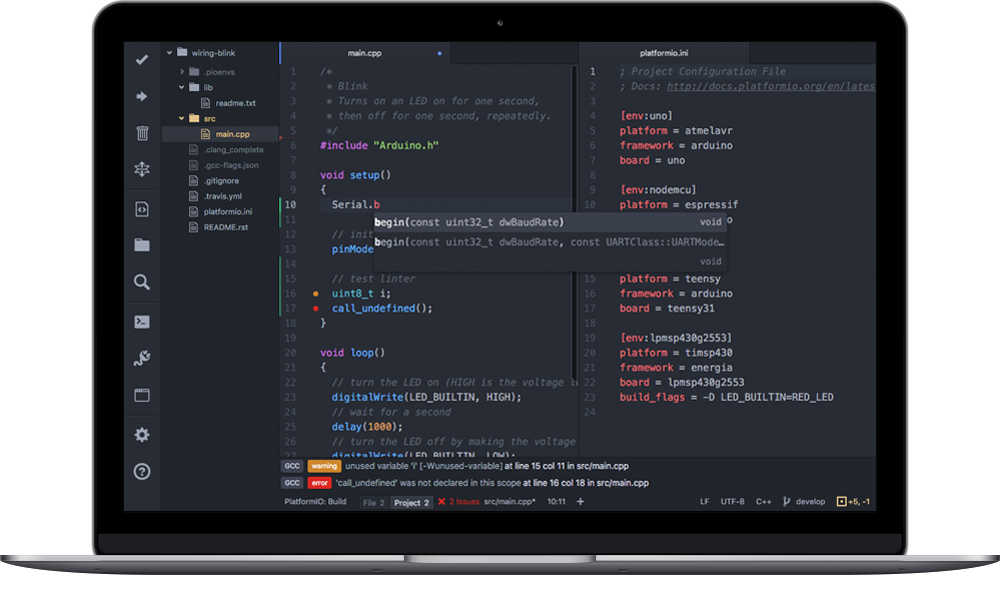
\includegraphics[width=0.9\linewidth]{../images/ide_arduino}
	\caption[IDE Arduino]{Interfaz de programación Arduino, con un fragmento de código. La interfaz permite compilar y cargar el ejecutable en la placa Arduino.}
	\label{fig:ide_arduino}
\end{figure}



\section{Organización del código fuente}

El código fuente del firmware queda distribuido en los siguientes ficheros:

\begin{itemize}
	
\item \texttt{Ardufocuser-config.h}: \textbf{Configuración}, así como el mapeo de pines y demás definiciones. 
\item \texttt{Ardufocuser-init.h}:   \textbf{Inicializa el sistema}, creando las instancias de los objetos utilizados, variables globales, contadores y demás estados.
\item \texttt{Ardufocuser-cmd.h}: \textbf{Comandos remotos}, junto con sus funciones callback asociadas.
\item \texttt{Ardufocuser-utils.h}: \textbf{Funciones de propósito general}, útiles en algunos de los módulos. 
\item \texttt{Ardufocuser.ino}: \textbf{Controlador principal}, incluye los ficheros anteriores, contiene las funciones \texttt{setup()}, \texttt{loop()} y \texttt{callbacks} de las interrupciones hardware y software (fragmento de código~\ref{lst:nucleo_firmware_ardufocuser}).

\item \texttt{library.json}: \textbf{Referencia a las bibliotecas de terceros}, catalogadas, y con referencias al sitio web y al desarrollador o equipo de desarrollo. Por seguridad también se incorporan al repositorio en el directorio \texttt{libs}.  


\end{itemize}

\begin{lstlisting}[language=cpp, caption={Núcleo implementación firmware  ardufocuser},label={lst:nucleo_firmware_ardufocuser}]
=======
\section{Implementación firmware}

En este capítulo se expone el trabajo relacionado con la programación a bajo nivel realizada sobre la electrónica propuesta en el capítulo Módulo Hardware.
Dado que la electrónica se basa en la plataforma Arduino, tal programación se realiza usando su propio lenguaje,  implementado en C/C++.

Este lenguaje se llama \textbf{Wiring} y se define a sí mismo como:

\textit{Entorno de programación de entradas/salidas de código abierto para explorar las artes electrónicas, los medios materiales, la enseñanza y el aprendizaje de la programación informática y creación de prototipos con electrónica.
}


\subsection{Diseño y Análisis}

Pasamos a determinar los requisitos que debe satisfacer nuestro firmware.
El requisito principales es claro, y consiste en ser capaz de controlar y manejar toda la información todos los periféricos  los datos que arrojan, ello se puede desglosar:

\begin{itemize}
	\item \textbf{Motor}, controla el movimiento, la velocidad, y la posición. 
	\item \textbf{Botones y potenciometos}, controla las pulsaciones y el cambio en el valor de los potenciometros, para controlar el dispositivo de forma manual. 
	\item \textbf{Pantalla LCD}, mostrar toda la información por pantalla.
	\item \textbf{Sensores}, recabar información del estado del dispositivo, temperatura, fines de recorrido.
	\item \textbf{Sesión persistente}, almacenar información de trabajo a otra.
	\item \textbf{API Serie}, interpretar y manejar comando vía mediante comunicación puerto serie, para permitir controlar el dispositivo desde un host.
\end{itemize}

Todo ello debe implementarse con una buena calidad permitiendo añadir más módulos y que se pueda cambiar fácilmente el repertorio de instrucciones de la API.

\subsection{Arquitectura firmware}


Para la programación del firmware sigo un diseño donde diferencio 4 bloques.


\begin{itemize}
	\item \textbf{Initializer}: Método \textbf{init} de la api de Arduino, que se ejecuta en primera instancia, prepara todo el entorno de ejecución, declarando las entradas, salidas,  reservando memoria, iniciar interrupciones, así como ejecutar rutinas como cargar sesión anterior o crear instancias a modo de singleton para manejador los diferentes periféricos. 
	\item \textbf{Controlador principal}: Bucle principal que se ejecuta periódicamente (el periodo no se puede modificar y lo marca la velocidad del reloj del micro), por lo tanto no es adecuado ejecutar rutinas con restricciones temporales fuertes, se corresponde con el método \textbf{loop}, se ocupa de manejar la mayoria de las entradas y salidas.
	\item \textbf{Interrupciones software}, se ejecutan en un periodo marcado por un timer, similar al loop pero con periodos fijo, se usa para rutinas con restricciones temporales fuertes.
	item \textbf{Interrupciones hardware}, se ejecutan rutinas ligadas directamente a eventos de entrada y salida en alguno de los pines habilitados para tal fin. 
\end{itemize}

Podemos ver un diagrama simplificado en la siguiente imagen.

\begin{figure}
\centering
\includegraphics[width=0.7\linewidth]{"../images/Arquitectura firmware"}
\caption{}
\label{fig:Arquitecturafirmware}
\end{figure}

\subsection{Módulo motores}

Para el control del motor, dado que debemos hacerlo con una gran precisión, hacemos uso de la libreria 
\textbf{AccelStepper} \cite{accelstp} 

\subsection{Módulo control remoto}

Para realizar el control remoto, hago uso de la comunicación serie que incorpora la placa Arduino.


El puerto serie envía la información mediante una secuencia de bits. Para ello se necesitan al menos dos conectores para realizar la comunicación de datos, RX (recepción) y TX (transmisión). 

En ocasiones veréis referirse a los puertos de serie como UART. La UART (universally asynchronous receiver/transmitter) es una unidad que incorporan ciertos procesadores, encargada de realiza la conversión de los datos a una secuencia de bits y transmitirlos o recibirlos a una velocidad determinada.

Los puertos serie están físicamente unidos a distintos pines, en Arduino UNO y Mini Pro los pines empleados son 0 (RX) y 1 (TX).


\begin{lstlisting}[language=C, caption={Ejemplo lectura y escritura puerto serie},label={lst:write_read_serial_port_sample}]

void setup(){
Serial.begin(9600);
}

void loop(){

}

void witeCharapter(char c){
Serial.println(c);
}

void readCharapter(){
if (Serial.available()>0){
input=Serial.read();
Serial.println(input);
}


\end{lstlisting}


Dado que tengo una cantidad de funciones a ejecutar mediante comandos, necesito formalizar un protocolo basado en mensajes preestablecidos. \\
Por seguir una nomenclatura, todos los comandos tienen el siguiente formato: \\


$ COMANDO?ARGUMENTO1?ARGUMENTO2  $

Y a continuación una lista de los comandos utilizados.


\begin{figure}[h]
	\centering
	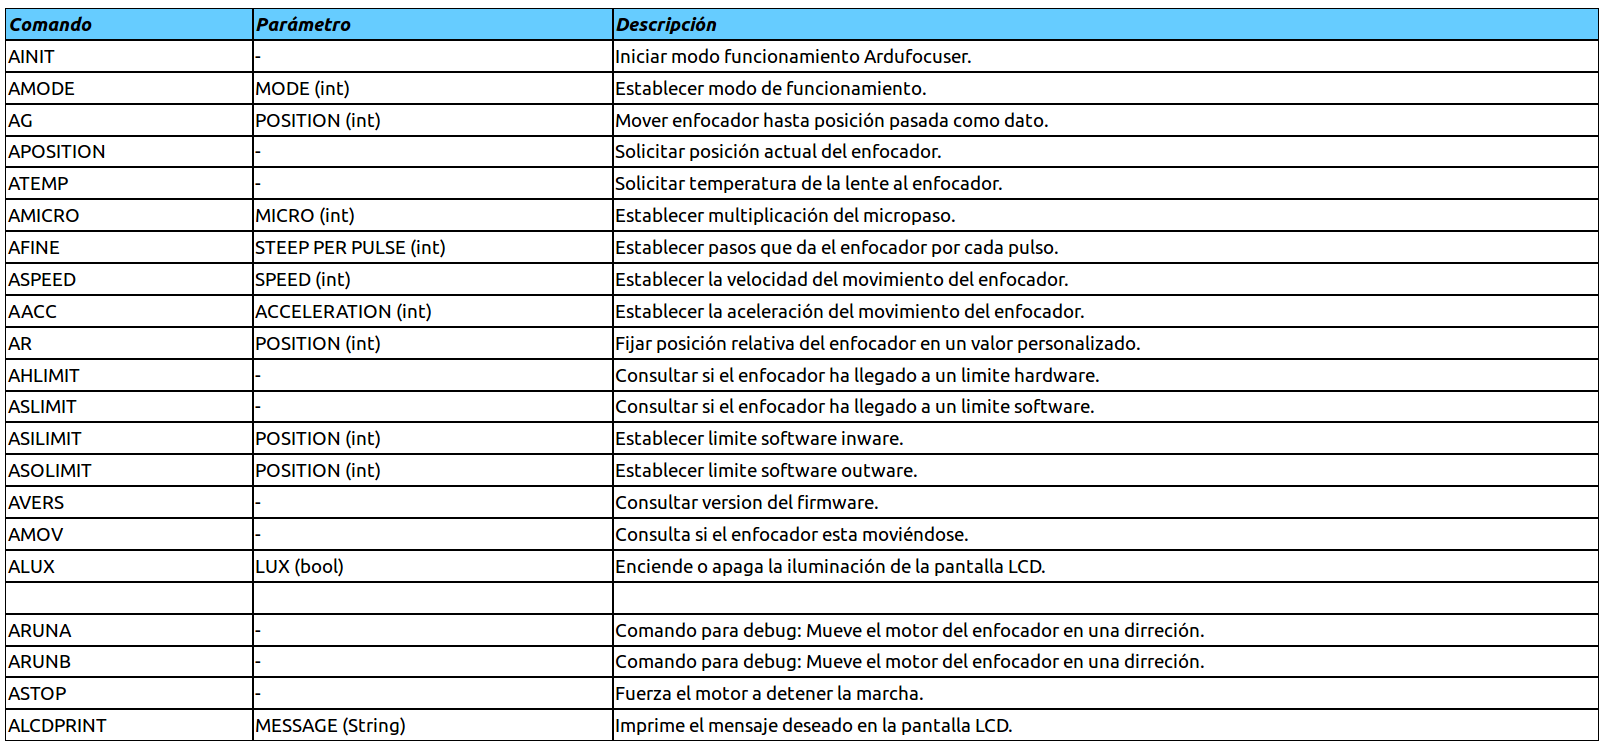
\includegraphics[width=1.1\linewidth]{../images/comando_ardufocuser}
	\caption{}
	\label{fig:comando_ardufocuser}
\end{figure}

Por regla general, todo comando tiene un mensaje de respuesta, bien indicando el nuevo estado del sistema que se ha cambiado (comandos escritura), bien información sobre el estado sobre el que solicitamos información (comandos lectura) o un ECHO del comando en algún otro caso.

\newpage


Con la experiencia y el trabajo, voy familiarizándome con la plataforma, conozco nuevas bibliotecas que me ayudan, nuevos periféricos,  así como mediante sesiones de refactorización, se consigue hacer código mantenible y modular. 

Es importante mencionar el uso de la herramienta \textbf{PlatformIO}, que se define a sí misma como un ecosistema abierto de desarrollo orientado a hardware. 


Tres son las características más sustanciales. 


- PlatformIO IDE: Un IDE orientado a la programación hardware, con funciones para facilitar la depuración, así como avisos para mejorar la calidad, totalmente configurado para compilar y cargar el programa directamente en una placa física, o en una placa virtual.

\begin{figure}
	\centering
	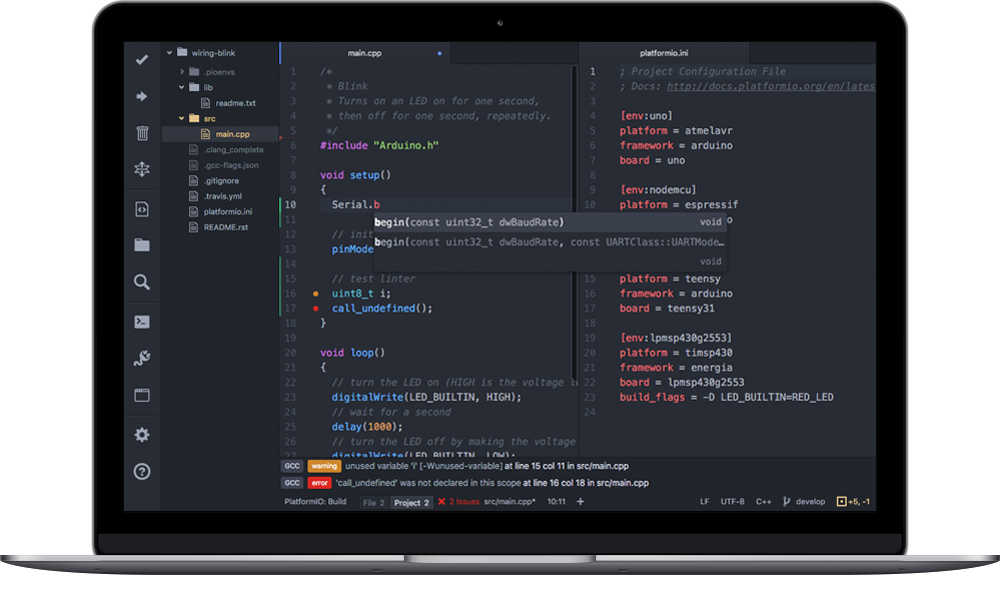
\includegraphics[width=0.7\linewidth]{../images/ide_arduino}
	\caption{}
	\label{fig:ide_arduino}
\end{figure}

- Terminal para realizar compilación en el cloud  para diferentes placas, así como permite compilación desde plataformas de integración continua como Travis CI.

- Gestor de bibliotecas y dependencias, tiene un repositorio con las bibliotecas más usadas, pudiendo buscar y actualizar rápidamente. 



El código fuente del firmware queda distribuido en los siguientes ficheros.

\begin{itemize}
	
\item $Ardufocuser-config.h$: Encapsula gran parte de la configuración, así como el mapeo de pines y demás definiciones. 
\item $Ardufocuser-init.h$: Inicializa el sistema, creando las instancias de los objetos utilizados, variables globales, contadores y demás estados.
\item $Ardufocuser-cmd.h$: Se definen los comandos remotos, junto con sus funciones callback asociadas.
\item $Ardufocuser-utils.h$: Incorpora algunas funciones de propósito general útiles en algunos de los módulos. 
\item $Ardufocuser.ino$: Es el script principal, incluye los ficheros anteriores, contiene las funciones setup(),  loop() y callback de las interrupciones hardware y software.

\item $library.json$: Hace referencia a las librerías de terceros, catalogadas, y con referencias al sitio web y al desarrollador o equipo de desarrollo. Por seguridad también las incorporo al repositorio en el directorio libs.  


\end{itemize}
\newpage
\begin{lstlisting}[language=C, caption={Núcleo implementación firmware  ardufocuser},label={lst:nucleo_firmware_ardufocuser }]

>>>>>>> c9f08dfe66521d4f0dba18e652f93a6a37a333aa
	void setup()
	{
		//Inicia comunicación serie.
		Serial.begin(9600);
		
		// Inicia pantalla LCD.
		lcd.begin();
		lcd.backlight();
		
		// Saludo inicial.
		welcome("   ARDUFOCUSER  ");
		
		// Velocidad y Aceletación inicial del motor.
		motor.setMaxSpeed(200);
		motor.setAcceleration(1000);
		
		//Iniciamos control Nunckuck
		chuck.begin();
		chuck.update();
		
<<<<<<< HEAD
		// Actualizamos con datos guardados en sesion 
		// anterior
		load_session();
		
		// Iniciamos interrupciones Software.
=======
		// Actualizamos con datos guardados en sesion anterior
		load_session();
		
		// Iniciamos interrupciones Software.
		// Gestiona movimiento del motor.
>>>>>>> c9f08dfe66521d4f0dba18e652f93a6a37a333aa
		Timer1.initialize(50);
		Timer1.attachInterrupt(timerFunction);
		
		// Inicia interrupciones hardware a la escucha.
		attachInterrupt ( 0, finA,RISING);
		attachInterrupt ( 1, finB,RISING);
		
		// Registramos y iniciamos comandos serie.
		registerCommand();
	}
<<<<<<< HEAD
=======
	
>>>>>>> c9f08dfe66521d4f0dba18e652f93a6a37a333aa
	void loop()
	{
		// Leemos nuevo comando serie.
		serial_cmd.readSerial();
<<<<<<< HEAD
		// Leemos control manual y sensores auxiliares.
		read_manual_controller();
		// Actualizamos LCD.
		update_lcd_display();
		// Leemos controles nunchuck.
		nunckuck_controller();
		// Almacenamos estados de forma persistente.
		save_current_session();
	}
\end{lstlisting}


\section{Pruebas}


Se han llevado a cabo \textbf{pruebas unitarias} de cada módulo en concreto. Estas consisten en ejecutar individualmente las funciones involucradas en cada uno de los módulos observando si el comportamiento es adecuado. 

Para ello hacemos uso de varios scripts adicionales:

\begin{itemize}
	\item \texttt{test-eeprom-mem}: Testea módulo de almacenamiento en memoria EEPROM. 
	\item \texttt{test-hardw-intrp}: Testea módulo de interrupciones hardware.
	\item \texttt{test-lcd}: Testea módulo de visualización en la pantalla LCD.
	\item \texttt{test-motor}: Testea módulo de control del motor.
	\item \texttt{test-nunchuck}: Testea módulo controlador del Nunchuck.
	\item \texttt{test-serial-comand}: Testea  módulo de comunicación serie. 
	\item \texttt{test-temp-sensor}: Testea  módulo del sensor de temperatura. 
	\item \texttt{test-poten}: Testea el módulo de lectura de los potenciómetros. 
\end{itemize}

La utilidad de estos script es inestimable, puesto que ayudan a detectar rápidamente posibles incidencias, tanto de \textbf{programación} como de \textbf{electrónica}. También ayudan a comprobar que los componentes que usamos en el montaje no tienen defectos de fábrica.



Adicionalmente se han llevado a cabo \textbf{pruebas de caja negra}, donde únicamente se tienen en cuenta las entradas que recibe el sistema y las salidas o respuestas que produce, sin preocuparnos del funcionamiento interno. Algunos de los casos de prueba que se han llevado a cabo se detallan en las tablas~\ref{caso_prueba_motor_api},\ref{caso_prueba_lcd_api} y \ref{caso_prueba_sesion}.


\begin{table}[h!]
	\centering

	\begin{tabular}{|l|l|}
		\hline
		ID caso de prueba             &  8 \\ \hline
		Nombre prueba                 &  Prueba ajustar posición enfocador mediante API serie. \\ \hline
		Autor de la prueba            &  José Miguel López \\ \hline
		Responsable diseño            &  José Miguel López \\ \hline
		\begin{tabular}[c]{@{}l@{}}Pasos y condiciones\\ de ejecución \end{tabular} &  \begin{tabular}[c]{@{}l@{}}
			- Conectamos el dispositivo a la alimentación. \\
			- Conectamos el dispositivo mediante USB a un PC. \\
			- Abrirnos un cliente serie (Arduino IDE - Monitor Serial) \\
			- Configuramos una velocidad de \textbf{9600 baud}. \\
			- Mandamos comando \textbf{AG?50} \\		
		\end{tabular} \\ \hline

		Resultado deseado             & \begin{tabular}[c]{@{}l@{}}
			 - El motor del enfocador se moverá hasta la posición 50 \\
			 - Periódicamente responderá con el comando\\APOSITION?X, 
			   siendo X la posición actual.     \\
			 - Cuando alcance la posición 50,   \\
			   responderá con el comando ASTOP? \\
		\end{tabular} \\ \hline
		
		Resultado obtenido            &  \begin{tabular}[c]{@{}l@{}}
			- El motor del enfocador se mueve hasta la posición 50 \\
			- Periódicamente responde con el comando\\APOSITION?X, 
			  siendo X la posición actual.     \\
			- Cuando alcanza la posición 50,   \\
			  responde con el comando ASTOP? \\
		\end{tabular} \\ \hline
		Estado caso de prueba         &  Éxito \\ \hline
		Errores asociados             &  Ninguno\\ \hline
		Comentario                    &  \\ \hline
	\end{tabular}
		\caption{Caso de prueba, ajustar posición enfocador mediante API serie.}
	\label{caso_prueba_motor_api}
\end{table}


\begin{table}[h!]
	\centering

	\begin{tabular}{|l|l|}
		\hline
		ID caso de prueba             &  8 \\ \hline
		Nombre prueba                 &  Prueba comando apagar iluminación LCD \\ \hline
		Autor de la prueba            &  José Miguel López \\ \hline
		Responsable diseño            &  José Miguel López \\ \hline
		\begin{tabular}[c]{@{}l@{}}Pasos y condiciones\\ de ejecución \end{tabular} &  \begin{tabular}[c]{@{}l@{}}
			- Conectamos el dispositivo a la alimentación. \\
			- Conectamos el dispositivo mediante USB a un PC. \\
			- Abrirnos un cliente serie (Arduino IDE - Monitor Serial) \\
			- Configuramos una velocidad de \textbf{9600 baud}. \\
			- Mandamos comando \textbf{ALUX?} \\		
		\end{tabular} \\ \hline
		Resultado deseado             & \begin{tabular}[c]{@{}l@{}}
			Se debe apagar la retroiluminación de la pantalla. \\
		\end{tabular} \\ \hline
		
		Resultado obtenido            &  \begin{tabular}[c]{@{}l@{}}
			Se apaga la iluminación de la pantalla. \\
		\end{tabular} \\ \hline
		Estado caso de prueba         &  Éxito\\ \hline
		Errores asociados             &  Ninguno\\ \hline
		Comentario                    &  \\ \hline
	\end{tabular}
		\caption{Caso de prueba, apagar iluminación LCD mediante API serie.}
	\label{caso_prueba_lcd_api}
\end{table}




\begin{table}[h!]
	\centering

	\begin{tabular}{|l|l|}
		\hline
		ID caso de prueba             &  9 \\ \hline
		Nombre prueba                 &  Prueba almacenamiento sesión \\ \hline
		Autor de la prueba            &  José Miguel López \\ \hline
		Responsable diseño            &  José Miguel López \\ \hline
		\begin{tabular}[c]{@{}l@{}}Pasos y condiciones\\ de ejecución \end{tabular} &  \begin{tabular}[c]{@{}l@{}}
			- Conectamos el dispositivo a la alimentación. \\
			- Modificamos velocidad al valor 5. \\
			- Movemos enfocador hasta la posición 120. \\ 
			- Desconectamos alimentación y USB. \\
			- Conectamos alimentación. \\						
		\end{tabular} \\ \hline
		Resultado deseado             & \begin{tabular}[c]{@{}l@{}}
			El dispositivo debe iniciar con velocidad 5 \\
			y posición del enfocador 120 \\
		\end{tabular} \\ \hline
		
		Resultado obtenido            &  \begin{tabular}[c]{@{}l@{}}
			El dispositivo inicia en la posición 120 y velocidad 10.
		\end{tabular} \\ \hline
		Estado caso de prueba         &  Error\\ \hline
		Errores asociados             &  No se almacena correctamente la velocidad. \\ \hline
		Comentario                    &  Se diagnostica error de almacenamiento.\\ \hline
	\end{tabular}
		\caption{Caso de prueba, los estados son persistentes de una sesión para otra}
	\label{caso_prueba_sesion}
\end{table} 
 




Por otro lado para asegurar que el firmware implementado permite ser compilado en las distintas placas hacemos uso del framework   \textbf{PlatformIO} \cite{patform}.


En el fragmento de código~\ref{lst:travis} se muestra un script \textbf{Travis CI} que se ha añadido al repositorio del firmware. En tal script se añaden los comandos necesarios para compilar el firmware en el cloud así como realizar un test completo del firmware, con la integración de todos los módulos (figura~\ref{fig:travis_ci}).


 

\begin{lstlisting}[language=python, caption={Script travis para realizar integración continua},label={lst:travis}]
=======
		
		// Leemos control manual y sensores auxiliares.
		read_manual_controller();
		
		// Actualizamos LCD.
		update_lcd_display();
		
		// Leemos controles nunchuck.
		nunckuck_controller();
		
		// Almacenamos estados de forma persistente 
		// para otra sesión.
		save_current_session();
	}



\end{lstlisting}


\section{Pruebas}

Además para asegurar que el firmware implementado, permite ser compilado en las distintas placas hacemos uso del framework   \textbf{PlatformIO} \cite{patform}.


- Buscador centralizado de bibliotecas, en los proyectos Arduino es uno de los problemas, dado que cada una de ellas puede provenir de una fuente totalmente diferente, con esta herramienta contamos con un solo lugar.

\newpage
\begin{lstlisting}[language=python, caption={Script travis para realizar integración continua},label={lst:write_read_serial_port_sample}]

>>>>>>> c9f08dfe66521d4f0dba18e652f93a6a37a333aa
language: python
python:
- "2.7"

install:
- python -c "$(curl -fsSL https://raw.githubusercontent.com/platformio/platformio/master/scripts/get-platformio.py)"
- wget https://github.com/josemlp91/ardufocuser_firmware/raw/master/Ardufocuser/libs/TimerOne.zip
- unzip TimerOne.zip
- wget https://github.com/josemlp91/ardufocuser_firmware/raw/master/Ardufocuser/libs/i2clcd.zip
- unzip i2clcd.zip
- wget https://github.com/josemlp91/ardufocuser_firmware/raw/master/Ardufocuser/libs/AccelStepper-1.49.zip
- unzip AccelStepper-1.49.zip
- wget https://github.com/josemlp91/ardufocuser_firmware/raw/master/Ardufocuser/libs/nunchuck.zip
- unzip nunchuck.zip

script:
- platformio ci Ardufocuser --lib="TimerOne" --lib="i2clcd" --lib="nunchuck" --lib="AccelStepper" --board=uno
<<<<<<< HEAD
\end{lstlisting}


\begin{center}
	\begin{figure}[h]	\centering
	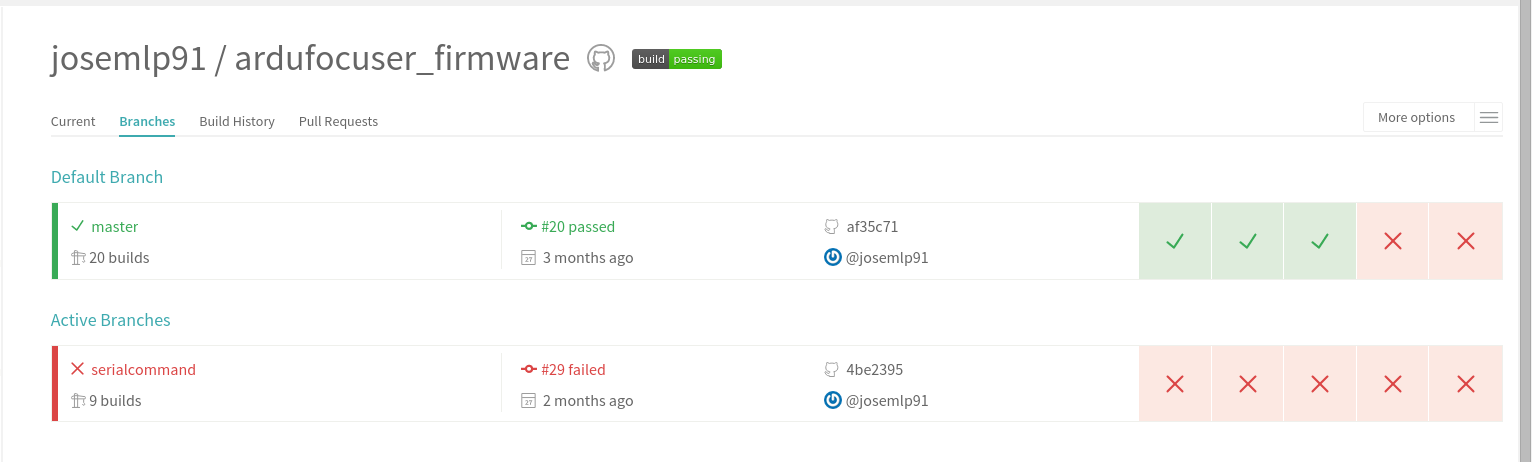
\includegraphics[width=1\linewidth]{../images/travis_ci}
	\caption[Ejecución tests Travis CI]{Ejecución del tests \textbf{Travis CI} tras realizar subidas al servidor de GitHub.}
	\label{fig:travis_ci}
\end{figure}
\end{center}






=======

\end{lstlisting}
>>>>>>> c9f08dfe66521d4f0dba18e652f93a6a37a333aa

